% =====================================================================
% Retrieval-Augmented Text-to-SQL with PEFT for Cross-Domain NBA Analytics
% Final write-up for COSI 115b -- Fundamentals of NLP II
% Author: Zixin (Stan) Wan
%
% Build (Overleaf or local TeX Live):
%   pdflatex final_writeup.tex
%   pdflatex final_writeup.tex   % twice for refs
%
% All figures (PDF) live in ./figures/. CSVs cited in the text live in ../eval/.
% =====================================================================

\documentclass[11pt,a4paper]{article}

\usepackage[margin=1in]{geometry}
\usepackage[utf8]{inputenc}
\usepackage[T1]{fontenc}
\usepackage{lmodern}
\usepackage{microtype}
\usepackage{graphicx}
\usepackage{booktabs}
\usepackage{array}
\usepackage{multirow}
\usepackage{caption}
\usepackage{subcaption}
\usepackage{pgfplots}
\usepackage{amsmath}
\usepackage{amssymb}
\usepackage{xcolor}
\usepackage{enumitem}
\usepackage{listings}
\usepackage{url}
\usepackage[hidelinks,colorlinks=true,linkcolor=blue!50!black,
            urlcolor=blue!50!black,citecolor=blue!50!black]{hyperref}
\pgfplotsset{compat=1.18}

% --- Listings (SQL) ---
\definecolor{lstBg}{HTML}{F7F7F7}
\definecolor{lstKw}{HTML}{1D428A}
\lstdefinelanguage{prettySQL}{
  morekeywords={SELECT,FROM,WHERE,GROUP,BY,ORDER,LIMIT,AS,AND,OR,JOIN,ON,
                COUNT,AVG,SUM,DISTINCT,HAVING,CASE,WHEN,THEN,ELSE,END,
                INNER,OUTER,LEFT,RIGHT,DESC,ASC,IN,NOT,EXISTS,IS,NULL},
  sensitive=false,
  morecomment=[l]{--},
  morestring=[b]',
}
\lstset{
  language=prettySQL,
  basicstyle=\ttfamily\footnotesize,
  keywordstyle=\color{lstKw}\bfseries,
  commentstyle=\color{gray}\itshape,
  stringstyle=\color{red!60!black},
  backgroundcolor=\color{lstBg},
  frame=single,
  rulecolor=\color{gray!40},
  numbers=none,
  breaklines=true,
  columns=fullflexible,
  keepspaces=true,
}

% --- Convenience macros ---
\newcommand{\codet}{\textsc{CodeT5+}}
\newcommand{\tfive}{\textsc{T5-base}}
\newcommand{\loraR}[1]{LoRA$_{r=#1}$}
\newcommand{\bestckpt}{\texttt{lora\_codet5p-220m\_r16\_nba\_nall\_s42}}
\newcommand{\spiderckpt}{\texttt{lora\_codet5p-220m\_r16\_bs4}}

\title{\bfseries Retrieval-Augmented Text-to-SQL with PEFT for\\
       Cross-Domain NBA Analytics}
\author{Zixin (Stan) Wan\\
        COSI 115b: Fundamentals of NLP II\\
        \textit{Track:} Applied \quad \textit{Focus:} Training}
\date{May 8, 2026}

% =====================================================================
\begin{document}
\maketitle

\begin{abstract}
\noindent
We build an end-to-end text-to-SQL system that maps English questions about an
NBA SQLite database into executable SQL. Spider~\cite{yu2018spider} is the
source-domain training corpus and a held-out 50-question NBA test split is the
target. Within the Applied~+~Training setup, we systematically compare full
fine-tuning, LoRA~\cite{hu2022lora}, and QLoRA~\cite{dettmers2023qlora} on
\tfive{} and \codet{}~\cite{wang2021codet5}, and we sweep three retrieval
backends (BM25, dense sentence-transformers + FAISS, and reciprocal-rank-fusion
hybrid) at $k\in\{1,3,5\}$. Our headline finding is that
\emph{in-domain adaptation data dominates retrieval choice}: with the full NBA
train split, oracle-schema execution accuracy reaches $0.46$ for the best
checkpoint, while end-to-end RAG with $\geq 0.92$ mean retrieval recall stalls at
$0.12$--$0.14$. A per-example recall-bin analysis shows \emph{retrieval is
necessary but not sufficient}: even when all gold tables are retrieved,
generation still fails on most NBA-specific questions, motivating
schema-conditioned decoding rather than further retriever tuning.
\end{abstract}

% =====================================================================
\section{Introduction}
\label{sec:intro}

This project translates natural-language questions about a single
NBA statistics database into executable SQL. The setup deliberately creates a
cross-domain transfer problem: training data is broad and heterogeneous
(Spider, $200$ databases), while deployment questions are from a narrow sports
schema with distinct vocabulary (e.g.\ \texttt{play\_by\_play},
\texttt{team\_name\_home}, \texttt{season\_id}~=~`22022') and query patterns.

Following the project specification, this is an \emph{Applied} project:
the deliverable is a runnable pipeline from question $\to$ SQL generation $\to$
SQLite execution $\to$ answer (with a Gradio demo, \texttt{src/demo.py}). The
\emph{focus} is \emph{Training}: I run controlled comparisons of multiple
adaptation strategies (full fine-tune, LoRA, QLoRA), of LoRA rank
($r\in\{4,8,16,32\}$), of two backbones (\tfive{} and \codet{}-220M), and of an
NBA few-shot \emph{adaptation curve} ($n\in\{0,10,20,70,150\}$). Two practical
questions drive the work:
\begin{enumerate}[leftmargin=*,itemsep=2pt]
\item Which parameter-efficient strategy gives the best tradeoff for domain
      transfer into NBA SQL?
\item Does schema retrieval (RAG over table schemas) improve downstream SQL
      correctness, and where does it break?
\end{enumerate}

The honest, somewhat uncomfortable answer is that
(1) \codet{}~+~LoRA~+~full NBA adaptation is the best practical choice, but
(2) RAG \emph{breaks} the system relative to oracle schema even at near-perfect
mean retrieval recall, because schema-conditioned generation fails to
disambiguate NBA-specific columns under partial context.

% =====================================================================
\section{Related Work}
\label{sec:related}

Modern text-to-SQL was standardised by Spider~\cite{yu2018spider}, a large
cross-domain benchmark with database splits that emphasise compositional
generalisation. Standard pipelines pair a pretrained encoder--decoder with
schema-conditioned decoding and report execution and exact-match accuracy.

Parameter-efficient fine-tuning (PEFT)~\cite{hu2022lora,dettmers2023qlora}
enables low-memory adaptation on commodity GPUs by training small adapters
instead of all model weights, which is essential for the single-GPU regime in
this work. \tfive{}~\cite{raffel2020t5} is the default seq2seq backbone;
\codet{}~\cite{wang2021codet5} additionally uses code identifier-aware
pre-training, which is a strong inductive bias for SQL output.

Retrieval-Augmented Generation (RAG)~\cite{lewis2020rag} originally targeted
open-domain QA but has been widely adapted to schema retrieval for text-to-SQL,
where a retriever selects a relevant subset of tables and only their schemas
are placed in the prompt. We use RAG strictly for \emph{schema selection} (no
external corpora), and we ablate retrieval quality (recall@$k$) against
downstream execution accuracy.

This project sits at the intersection of these three lines: Spider
pre-training, PEFT comparisons, and RAG schema retrieval, all evaluated on a
fixed NBA hold-out split with execution-grounded metrics.

% =====================================================================
\section{Data}
\label{sec:data}

\paragraph{Spider (source).}
We use the official HuggingFace mirror \texttt{xlangai/spider}: 10{,}181
question/SQL pairs over 200 databases and 138 domains. Spider supplies the
heterogeneous source supervision; for cost reasons our Spider \emph{evaluation}
slice is the first 200 dev examples (per-database SQLite paths required for
execution accuracy on Spider were not wired up, so Spider numbers are reported
as exact-match only; see Section~\ref{sec:spider-controls}).

\paragraph{NBA (target).}
A SQLite database is built from the open-source
\href{https://github.com/mpope9/nba-sql}{nba-sql} pipeline ($\sim$15 NBA tables
covering players, teams, games, draft, play-by-play, line scores, and
combine stats). We hand-author \textbf{200 question/SQL pairs}
(\texttt{data/nba/nba\_questions.json}) stratified by Spider-style difficulty
\{\texttt{easy}, \texttt{medium}, \texttt{hard}, \texttt{extra\_hard}\}, with
each example annotated with its gold \texttt{tables\_used}, used both for the
oracle-schema upper bound and for retrieval recall@$k$.

\paragraph{Train/test protocol.}
We freeze a deterministic 150/50 train/test split
(\texttt{data/nba/nba\_split.json}). The 50-question test partition is held
out across every NBA experiment in this report; the 150-question train
partition feeds the few-shot adaptation curve at sizes
$n\in\{10,20,70,\text{all}{=}150\}$. The split is created once and pickled, so
all comparisons are directly comparable.

\paragraph{Schema documents (for retrieval).}
For RAG, each NBA table is rendered into a single ``document'' by
\texttt{src/data\_utils.build\_nba\_schema\_documents}: the table name plus a
Spider-style serialised column list with normalised types. The same documents
are indexed by all three retrieval backends, so retrieval differences come from
the scoring function and not from the document corpus.

% =====================================================================
\section{Methods}
\label{sec:methods}

The pipeline has four code-level components: training (\texttt{src/train.py}),
NBA adaptation (\texttt{src/train\_nba.py}), retrieval (\texttt{src/rag.py}),
and evaluation (\texttt{src/evaluate.py}). All four log run configurations to
disk for reproducibility.

\subsection{Base models and training regimes}
\label{sec:methods-train}

Implemented in \texttt{src/train.py}:
\begin{itemize}[leftmargin=*,itemsep=2pt]
  \item \textbf{Full fine-tune} (\texttt{--method full}) -- updates all
        parameters of \tfive{} or \codet{}.
  \item \textbf{LoRA}~\cite{hu2022lora} (\texttt{--method lora}, rank sweep
        $r\in\{4,8,16,32\}$) -- trains low-rank update matrices in attention
        and feed-forward projections; base weights frozen.
  \item \textbf{QLoRA}~\cite{dettmers2023qlora} (\texttt{--method qlora}) --
        4-bit NF4 base + LoRA adapters on top.
\end{itemize}
Each run writes \texttt{run\_config.json} (model, method, rank, learning rate,
batch size, gradient-accumulation steps, seed, mixed-precision flag) so the
final results table can be filtered and joined deterministically. We use
\texttt{seed=42}, \texttt{lr=1e-4}, batch~4 with grad-accum~2 unless otherwise
noted; mixed precision is bf16 when supported, else fp16.

\subsection{NBA domain adaptation}
\label{sec:methods-adapt}

\texttt{src/train\_nba.py} continues from a Spider-trained PEFT checkpoint and
fine-tunes the LoRA adapter on a subsample of the NBA train partition. A
critical fix discovered late in the project: \emph{merging} the LoRA into the
base before NBA adaptation and then full-fine-tuning the merged model on
$n\leq 70$ examples produced catastrophic forgetting (NBA execution accuracy
$=0.00$, generations collapsed to filler tokens). The current pipeline keeps
the adapter loaded as PEFT during NBA training (\texttt{is\_trainable=True}),
trains only the LoRA parameters, and merges with \texttt{merge\_and\_unload()}
\emph{after} training when saving \texttt{final/}. This recovered the few-shot
curve in Section~\ref{sec:fewshot}.

\subsection{Inference and three schema modes}
\label{sec:methods-eval}

\texttt{src/evaluate.py} supports three schema-input modes:
\begin{enumerate}[leftmargin=*,itemsep=2pt]
\item \textbf{Full schema} -- every NBA table's serialised schema in the prompt.
\item \textbf{Oracle tables} (\texttt{--oracle-tables}) -- only the gold
      \texttt{tables\_used} schemas; this is the perfect-retrieval upper
      bound.
\item \textbf{RAG} (\texttt{--use-rag --rag-backend \{dense,bm25,hybrid\}\\
      --top-k}) -- only the schemas of the retriever's top-$k$ tables.
\end{enumerate}
NBA evaluation defaults to \texttt{--split test} (the 50-question hold-out)
to prevent leakage. All RAG runs additionally log per-example
\texttt{retrieval\_recall} and \texttt{perfect\_retrieval} into the result
JSON, which feeds the recall-bin analysis in
Section~\ref{sec:rag-bins}.

Decoding uses beam search with $8$ beams, \texttt{max\_length}=256, and no
$n$-gram repetition restriction (SQL legitimately repeats tokens like
\texttt{home}, \texttt{home}). Execution accuracy compares the sorted result
sets of predicted vs gold SQL on the live SQLite (5\,s timeout); exact match
is lowercase + whitespace-normalised and is reported as a strict secondary.

\subsection{Three retrieval backends}
\label{sec:methods-retrieval}

All retrievers index the same per-table documents from
Section~\ref{sec:data}. Implementation lives in \texttt{src/rag.py}; a small
factory (\texttt{get\_schema\_retriever(backend)}) hides the implementation
behind a \texttt{retrieve(question, top\_k)} interface.

\begin{itemize}[leftmargin=*,itemsep=2pt]
  \item \textbf{Dense}: \texttt{sentence-transformers}/\texttt{all-MiniLM-L6-v2}
        embeddings normalised to unit norm, indexed in \texttt{faiss-cpu}
        with inner product (cosine).
  \item \textbf{BM25}: \texttt{rank\_bm25.BM25Okapi} over a simple
        whitespace/regex tokenisation; the table name is repeated inside the
        document text to boost lexical overlap.
  \item \textbf{Hybrid}: reciprocal rank fusion (RRF, $k_{\text{rrf}}=60$) of
        the \emph{full} BM25 and dense rankings; then take top-$k$. We chose
        RRF over learned-weight fusion because it has no hyper-parameters to
        tune on this small benchmark and is the standard
        information-retrieval baseline.
\end{itemize}

\subsection{End-to-end RAG protocol (two checkpoints)}
\label{sec:methods-rag-protocol}

To separate ``retrieval helps'' from ``adaptation helps,'' the end-to-end
RAG sweep runs both
\spiderckpt{} (Spider-only, \emph{no} NBA adaptation) and
\bestckpt{} (the same architecture after full NBA adaptation). The driver is
\texttt{scripts/run\_rag\_retrieval\_ablation.py}, which produces
\texttt{eval/rag\_retrieval\_summary.csv} (recall-only),
\texttt{eval/rag\_e2e\_summary.csv} ($18$ end-to-end runs $=2\,\text{ckpts}\times
3\,\text{backends}\times 3\,k$), and
\texttt{eval/rag\_recall\_bins\_summary.csv}.

% =====================================================================
\section{Results}
\label{sec:results}

All NBA numbers are on the held-out $n=50$ test split. Confidence intervals
in tables are bootstrap 95\% CIs computed by
\texttt{src/build\_results\_report.py} (1{,}000 resamples).

\subsection{Spider source-domain controls}
\label{sec:spider-controls}

Table~\ref{tab:spider} reports exact match on a 200-example Spider dev slice
(execution accuracy on Spider was not wired up due to per-database
SQLite-path bookkeeping; we keep the Spider table strictly as a relative
\emph{control} for source-domain learning).

\begin{table}[h]
\centering
\caption{Spider dev slice ($n=200$), exact match $\pm$ 95\% bootstrap CI.
Execution accuracy not run on Spider in this protocol.}
\label{tab:spider}
\small
\begin{tabular}{l l c c}
\toprule
Model & Method & Exact match & 95\% CI \\
\midrule
\codet{}-220M (bs4) & LoRA $r{=}16$       & \textbf{0.325} & [0.260, 0.390] \\
\codet{}-220M       & LoRA $r{=}16$       & 0.290          & [0.230, 0.355] \\
\tfive{}            & Full fine-tune      & 0.265          & [0.205, 0.330] \\
\tfive{}            & LoRA $r{=}32$       & 0.215          & [0.160, 0.275] \\
\tfive{}            & QLoRA               & 0.175          & [0.120, 0.230] \\
\tfive{}            & LoRA $r{=}8$        & 0.145          & [0.095, 0.195] \\
\tfive{}            & LoRA $r{=}16$       & 0.120          & [0.080, 0.165] \\
\tfive{}            & LoRA $r{=}4$        & 0.070          & [0.035, 0.105] \\
\bottomrule
\end{tabular}
\end{table}

\begin{figure}[h]
\centering
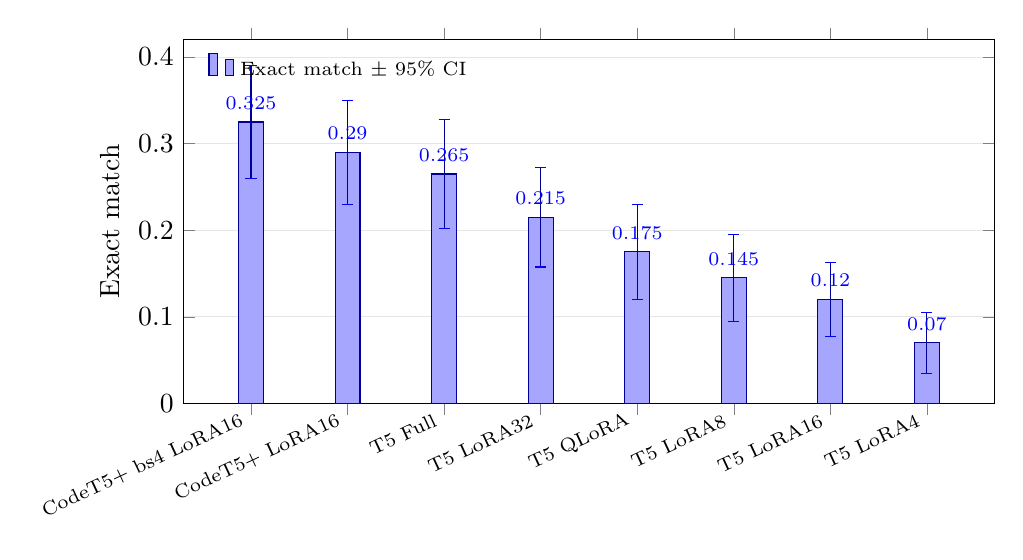
\begin{tikzpicture}
\begin{axis}[
  width=0.98\linewidth,
  height=6.2cm,
  ybar,
  bar width=9pt,
  ymin=0, ymax=0.42,
  ylabel={Exact match},
  symbolic x coords={CodeT5+ bs4 LoRA16,CodeT5+ LoRA16,T5 Full,T5 LoRA32,T5 QLoRA,T5 LoRA8,T5 LoRA16,T5 LoRA4},
  xtick=data,
  xticklabel style={rotate=25,anchor=east,font=\scriptsize},
  ymajorgrids=true,
  grid style={gray!20},
  legend style={at={(0.02,0.98)},anchor=north west,font=\scriptsize,draw=none,fill=none},
  nodes near coords,
  nodes near coords style={font=\scriptsize, /pgf/number format/fixed, /pgf/number format/precision=3},
  every node near coord/.append style={yshift=1pt}
]
\addplot+[
  fill=blue!35,
  draw=blue!60!black,
  error bars/.cd,
  y dir=both,
  y explicit
] coordinates {
  (CodeT5+ bs4 LoRA16,0.325) +- (0,0.065)
  (CodeT5+ LoRA16,0.290) +- (0,0.060)
  (T5 Full,0.265) +- (0,0.0625)
  (T5 LoRA32,0.215) +- (0,0.0575)
  (T5 QLoRA,0.175) +- (0,0.055)
  (T5 LoRA8,0.145) +- (0,0.050)
  (T5 LoRA16,0.120) +- (0,0.0425)
  (T5 LoRA4,0.070) +- (0,0.035)
};
\legend{Exact match $\pm$ 95\% CI}
\end{axis}
\end{tikzpicture}
\caption{Spider controls from Table~\ref{tab:spider}: exact match with 95\% bootstrap CI.}
\label{fig:spider-controls-ci}
\end{figure}

The two \codet{} runs lead by a comfortable margin, consistent with the
code-aware pre-training. Within \tfive{}, full fine-tune $>$ rank-32 LoRA $>$
QLoRA $>$ smaller LoRA ranks; the gap from $r{=}16$ to $r{=}32$ is real but
modest. These controls justify selecting \codet{}~+~LoRA $r{=}16$ as the
backbone for NBA adaptation and RAG.

\subsection{NBA few-shot adaptation curve}
\label{sec:fewshot}

Table~\ref{tab:fewshot} sweeps NBA train size for both backbones, oracle-tables
mode (the upper bound that isolates ``can the model write NBA SQL given
correct schema?''). Numbers are from \texttt{eval/fewshot\_curve.csv}.

\begin{table}[h]
\centering
\caption{NBA test execution accuracy (n{=}50), oracle-tables mode, by
adaptation size $n$. CIs are 95\% bootstrap. Bold = best per backbone.}
\label{tab:fewshot}
\small
\begin{tabular}{l r c c}
\toprule
Backbone (LoRA $r{=}16$) & $n_{\text{train}}$ & Exec acc.\ (CI) & Exact (CI) \\
\midrule
\multirow{5}{*}{\codet{}-220M}
    & 0   & 0.10 [0.02, 0.18]  & 0.00 [0.00, 0.00] \\
    & 10  & 0.06 [0.00, 0.12]  & 0.02 [0.00, 0.06] \\
    & 20  & 0.14 [0.06, 0.24]  & 0.06 [0.00, 0.14] \\
    & 70  & 0.18 [0.08, 0.30]  & 0.06 [0.00, 0.14] \\
    & all & \textbf{0.24} [0.12, 0.36] & \textbf{0.16} [0.06, 0.26] \\
\midrule
\multirow{5}{*}{\tfive{}}
    & 0   & 0.04 [0.00, 0.10]  & 0.02 [0.00, 0.08] \\
    & 10  & 0.02 [0.00, 0.06]  & 0.00 [0.00, 0.00] \\
    & 20  & 0.02 [0.00, 0.06]  & 0.00 [0.00, 0.00] \\
    & 70  & 0.10 [0.02, 0.20]  & 0.06 [0.00, 0.14] \\
    & all & \textbf{0.12} [0.04, 0.22] & \textbf{0.10} [0.02, 0.20] \\
\bottomrule
\end{tabular}
\end{table}

\begin{figure}[h]
\centering
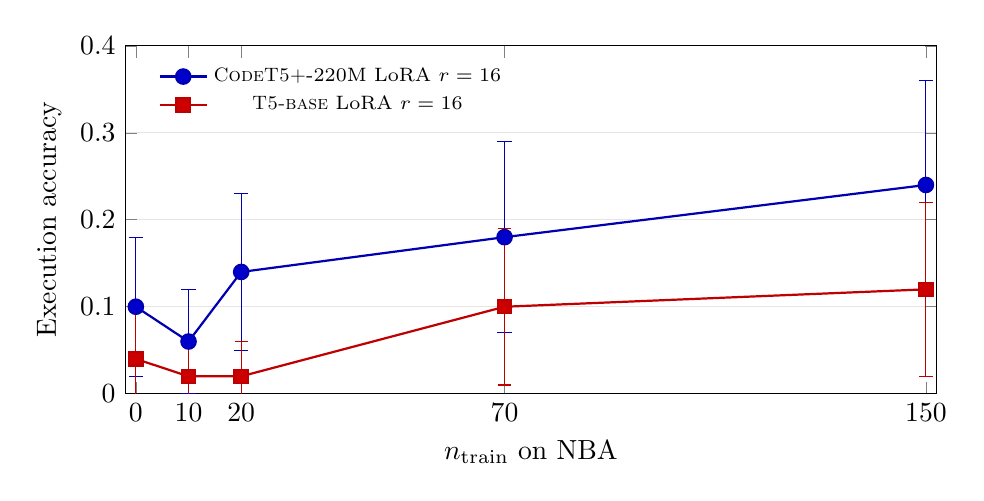
\begin{tikzpicture}
\begin{axis}[
  width=0.98\linewidth,
  height=6.0cm,
  ymin=0, ymax=0.40,
  xmin=-2, xmax=152,
  xlabel={$n_{\text{train}}$ on NBA},
  ylabel={Execution accuracy},
  xtick={0,10,20,70,150},
  ymajorgrids=true,
  grid style={gray!20},
  legend style={at={(0.03,0.97)},anchor=north west,font=\scriptsize,draw=none,fill=none}
]
\addplot+[
  color=blue!70!black,
  mark=*,
  mark size=2.6pt,
  thick,
  error bars/.cd,
  y dir=both,
  y explicit
] coordinates {
  (0,0.10) +- (0,0.08)
  (10,0.06) +- (0,0.06)
  (20,0.14) +- (0,0.09)
  (70,0.18) +- (0,0.11)
  (150,0.24) +- (0,0.12)
};
\addlegendentry{\codet{}-220M LoRA $r=16$}

\addplot+[
  color=red!75!black,
  mark=square*,
  mark size=2.4pt,
  thick,
  error bars/.cd,
  y dir=both,
  y explicit
] coordinates {
  (0,0.04) +- (0,0.06)
  (10,0.02) +- (0,0.04)
  (20,0.02) +- (0,0.04)
  (70,0.10) +- (0,0.09)
  (150,0.12) +- (0,0.10)
};
\addlegendentry{\tfive{} LoRA $r=16$}
\end{axis}
\end{tikzpicture}
\caption{NBA few-shot adaptation curve from Table~\ref{tab:fewshot}: execution accuracy with 95\% bootstrap CI (all = 150 examples).}
\label{fig:fewshot-exec-ci}
\end{figure}

The headline finding for the \emph{Training} focus: \codet{} adapts more
sample-efficiently than \tfive{} (the gap at $n{=}\text{all}$ is 0.24 vs 0.12
in execution accuracy, with overlapping but clearly shifted CIs), and
\codet{}'s execution accuracy more than doubles between $n{=}20$ and
$n{=}\text{all}$. There is also an unsurprising small dip at $n{=}10$
(adapter starts overfitting before learning the domain), an effect the
LoRA-only fix in Section~\ref{sec:methods-adapt} significantly damped.

A separate, $n{=}\text{all}$, longer-trained \bestckpt{} checkpoint (used as
the RAG e2e backbone in the next section) reaches \textbf{exec 0.46 / exact
0.42} on the same test split with oracle tables; this is the upper bound the
RAG section is judged against.

\subsection{Retrieval-only quality}
\label{sec:rag-retrieval}

Table~\ref{tab:retrieval} evaluates the three retrievers on the same NBA
\emph{test} questions (recall is undefined when \texttt{tables\_used} is
empty; those questions are excluded). Mean recall and \emph{perfect-retrieval}
rate (all gold tables retrieved) come from
\texttt{eval/rag\_retrieval\_summary.csv}.

\begin{table}[h]
\centering
\caption{Retrieval-only on NBA test ($n=50$). Mean recall@$k$ and rate of
``perfect retrieval'' (all gold tables in top-$k$).}
\label{tab:retrieval}
\small
\begin{tabular}{l r c c}
\toprule
Backend & $k$ & Mean recall & Perfect rate \\
\midrule
Dense   & 1 & 0.17 & 0.14 \\
Dense   & 3 & 0.74 & 0.72 \\
Dense   & 5 & 0.85 & 0.84 \\
\midrule
BM25    & 1 & 0.24 & 0.24 \\
BM25    & 3 & 0.44 & 0.42 \\
BM25    & 5 & 0.94 & 0.94 \\
\midrule
Hybrid  & 1 & \textbf{0.37} & \textbf{0.36} \\
Hybrid  & 3 & \textbf{0.92} & \textbf{0.90} \\
Hybrid  & 5 & \textbf{0.99} & \textbf{0.98} \\
\bottomrule
\end{tabular}
\end{table}

Hybrid (RRF over BM25 and dense full rankings) wins at every $k$. BM25 alone
catches up at $k=5$ and slightly beats dense ($0.94$ vs $0.85$ mean recall),
which reflects the lexical overlap between question text (e.g.\
``\texttt{free throw percentage in playoffs}'') and column names (e.g.\
\texttt{ft\_pct}, \texttt{season\_type}); dense overweights paraphrases and
misses these shortcuts. The interesting consequence is that \emph{retrieval
quality is essentially solved at $k\geq 3$ by hybrid}, which sets up the
next section.

\subsection{End-to-end RAG: retrieval is necessary but not sufficient}
\label{sec:rag-e2e}

Table~\ref{tab:rag-e2e} reports execution accuracy for all
$2\,\text{checkpoints}\times 3\,\text{backends}\times 3\,k$ end-to-end runs
(\texttt{eval/rag\_e2e\_summary.csv}). Compare each row against the
oracle-tables upper bound for the same checkpoint
(\spiderckpt{}: $\sim$0.10; \bestckpt{}: \textbf{0.46}).

\begin{table}[h]
\centering
\caption{End-to-end RAG: NBA test execution accuracy by checkpoint, retriever,
and $k$. Oracle-tables upper bounds: $\sim$0.10 (Spider-only),
\textbf{0.46} (NBA-adapted).}
\label{tab:rag-e2e}
\small
\begin{tabular}{l l r c c}
\toprule
Checkpoint & Backend & $k$ & Exec acc.\ & Exact \\
\midrule
\multirow{9}{*}{\bestckpt{} (NBA-adapted)}
    & Dense  & 1 & 0.08 & 0.06 \\
    & Dense  & 3 & 0.08 & 0.08 \\
    & Dense  & 5 & 0.08 & 0.08 \\
    & BM25   & 1 & 0.10 & 0.04 \\
    & BM25   & 3 & \textbf{0.14} & 0.12 \\
    & BM25   & 5 & \textbf{0.14} & 0.12 \\
    & Hybrid & 1 & 0.10 & 0.08 \\
    & Hybrid & 3 & \textbf{0.14} & 0.12 \\
    & Hybrid & 5 & 0.12 & 0.12 \\
\midrule
\multirow{9}{*}{\spiderckpt{} (Spider-only)}
    & Dense  & 1 & 0.06 & 0.00 \\
    & Dense  & 3 & 0.08 & 0.00 \\
    & Dense  & 5 & 0.08 & 0.00 \\
    & BM25   & 1 & 0.06 & 0.00 \\
    & BM25   & 3 & 0.08 & 0.00 \\
    & BM25   & 5 & 0.08 & 0.00 \\
    & Hybrid & 1 & 0.08 & 0.00 \\
    & Hybrid & 3 & 0.08 & 0.00 \\
    & Hybrid & 5 & \textbf{0.10} & 0.00 \\
\bottomrule
\end{tabular}
\end{table}

Two observations are worth emphasising:

\begin{enumerate}[leftmargin=*,itemsep=2pt]
\item \textbf{Adaptation $\gg$ retrieval method.} For the NBA-adapted
      checkpoint, switching from the worst RAG cell (dense, $k=1$, $0.08$) to
      the best (BM25 or hybrid, $k=3$, $0.14$) gains $+0.06$. For the
      Spider-only checkpoint, the best RAG cell is $0.10$. The total spread
      from \emph{any} RAG configuration is small compared to the
      $0.46-0.14 = 0.32$ gap to the oracle upper bound on the
      adapted model.
\item \textbf{High recall does not translate.} Hybrid at $k=5$ achieves
      \emph{mean recall $0.99$ and perfect retrieval $0.98$} on test
      (Table~\ref{tab:retrieval}), but exec accuracy is only $0.12$ for the
      adapted model and $0.10$ for the Spider model. The bottleneck is no
      longer ``missing tables.''
\end{enumerate}

Figure~\ref{fig:recall-vs-exec} plots mean retrieval recall against execution
accuracy with one panel per checkpoint, and Figure~\ref{fig:bars-k3} shows the
backend comparison at $k=3$. The two figures together summarise the
``RAG breaks'' message: recall climbs cleanly into the high-0.9s, but exec
accuracy plateaus near the bottom.

\begin{figure}[h]
\centering
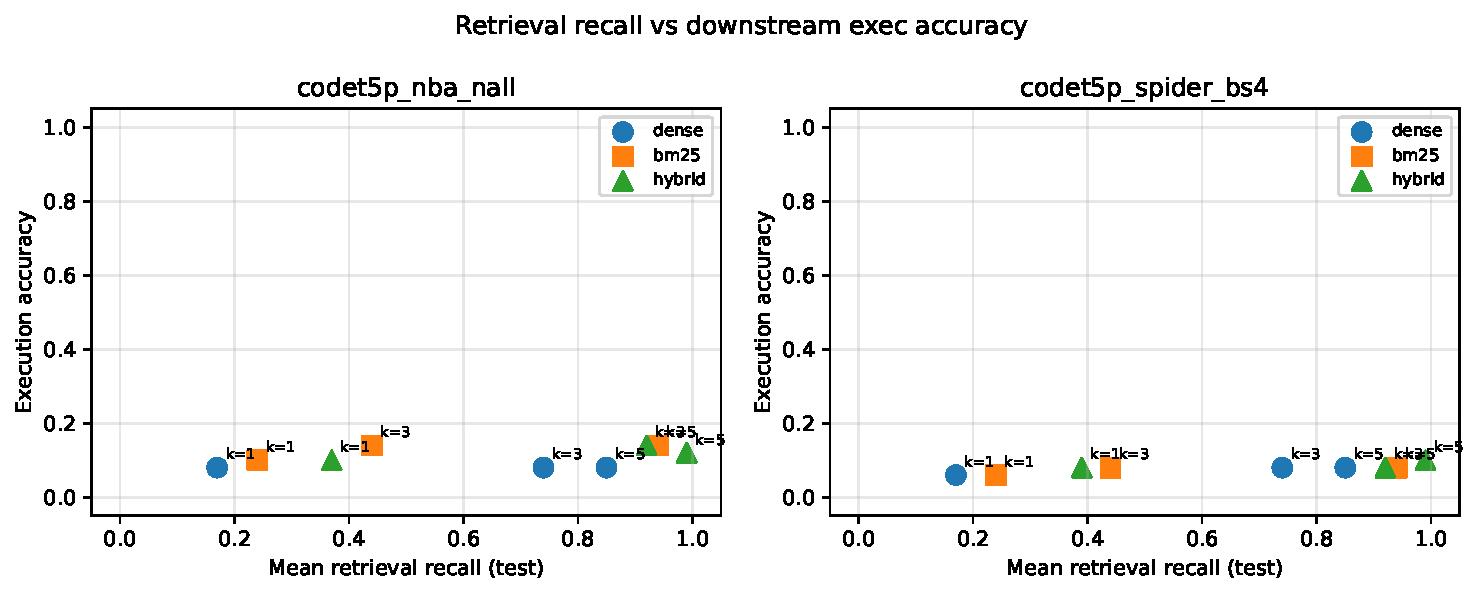
\includegraphics[width=\linewidth]{figures/rag_recall_vs_exec.pdf}
\caption{Per-run mean retrieval recall (x) vs NBA test execution accuracy (y),
faceted by checkpoint. Marker shape encodes retrieval backend; annotations
show $k$. Even when hybrid reaches near-perfect recall on the right edge of
each panel, downstream exec accuracy stays in the 0.08--0.14 band, far from
the oracle upper bound (0.46 for the NBA-adapted panel).}
\label{fig:recall-vs-exec}
\end{figure}

\begin{figure}[h]
\centering
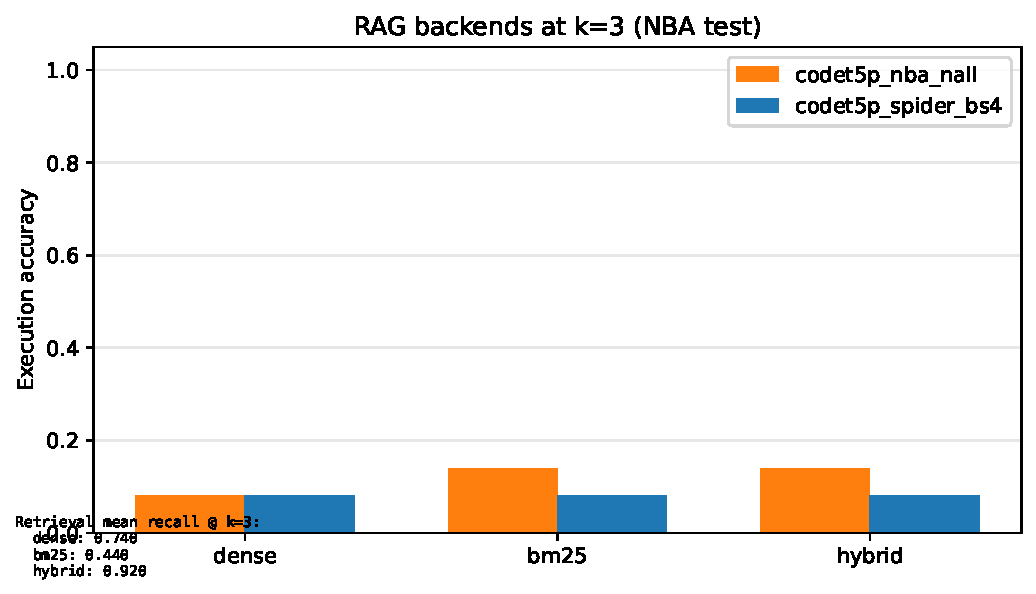
\includegraphics[width=0.85\linewidth]{figures/rag_backend_bars_k3.pdf}
\caption{NBA test execution accuracy at $k=3$ by retrieval backend, grouped by
checkpoint. The retrieval-mean-recall annotations match Table~\ref{tab:retrieval}
(BM25 $0.44$, dense $0.74$, hybrid $0.92$ at $k=3$).}
\label{fig:bars-k3}
\end{figure}

\subsection{Recall bins: a threshold effect, not a smooth gradient}
\label{sec:rag-bins}

Table~\ref{tab:bins} stratifies test examples by per-question retrieval
recall into three bins ($<0.4$, $0.4$--$0.7$, $>0.7$) and reports execution
rate within each bin, on the NBA-adapted checkpoint
(\texttt{eval/rag\_recall\_bins\_summary.csv}).

\begin{table}[h]
\centering
\caption{NBA-adapted checkpoint: execution rate stratified by per-example
retrieval recall, by retrieval backend and $k$. Empty cells indicate zero
examples in that bin (`--`).}
\label{tab:bins}
\small
\begin{tabular}{l c r c r c r c}
\toprule
        &     & \multicolumn{2}{c}{recall $<0.4$}
              & \multicolumn{2}{c}{recall $0.4$--$0.7$}
              & \multicolumn{2}{c}{recall $>0.7$} \\
\cmidrule(lr){3-4}\cmidrule(lr){5-6}\cmidrule(lr){7-8}
Backend & $k$ & $n$ & exec & $n$ & exec & $n$ & exec \\
\midrule
Dense   & 1 & 40 & 0.00 & 3 & 0.00 & 7  & \textbf{0.57} \\
Dense   & 3 & 12 & 0.00 & 2 & 0.00 & 36 & 0.11 \\
Dense   & 5 & 7  & 0.00 & 1 & 0.00 & 42 & 0.10 \\
BM25    & 1 & 38 & 0.00 & 0 & --   & 12 & \textbf{0.42} \\
BM25    & 3 & 27 & 0.00 & 2 & 0.00 & 21 & \textbf{0.33} \\
BM25    & 5 & 3  & 0.00 & 0 & --   & 47 & 0.15 \\
Hybrid  & 1 & 31 & 0.00 & 1 & 0.00 & 18 & 0.28 \\
Hybrid  & 3 & 3  & 0.00 & 2 & 0.00 & 45 & 0.16 \\
Hybrid  & 5 & 0  & --   & 1 & 0.00 & 49 & 0.12 \\
\bottomrule
\end{tabular}
\end{table}

There are two regularities. First, the low-recall bin
(recall~$<0.4$) is essentially \emph{always 0\% exec} -- if the retriever
misses gold tables, generation cannot recover. Second, the high-recall bin
(recall~$>0.7$) drops noticeably as $k$ grows: BM25 at $k=1$ on the perfectly
retrieved subset is $0.42$, but at $k=5$ it falls to $0.15$. The drop is a
\emph{distractor effect}: more candidate tables in the prompt (some
plausible but wrong, e.g.\ \texttt{game\_summary} vs \texttt{game}) push the
decoder toward the wrong join. This is exactly the threshold effect
hypothesised in the project todo and is the cleanest piece of evidence for the
``RAG breaks the system'' framing.

\subsection{Failure-case sample}
\label{sec:failures}

Table~\ref{tab:failures} samples 10 failed examples from \bestckpt{} with
dense $k=3$ (\texttt{internal\_docs/rag\_failure\_cases.md}), categorised as
\emph{retrieval\_miss} (gold tables not all retrieved) vs \emph{gen\_error}
(perfect retrieval, wrong SQL). The split is exactly 5/5 in this small sample,
mirroring the bin analysis: half the failures are upstream of generation,
half are not.

\begin{table}[h]
\centering
\caption{Sampled failures from \bestckpt{} with dense $k=3$. Truncated for
space. Full table in \texttt{internal\_docs/rag\_failure\_cases.md}.}
\label{tab:failures}
\scriptsize
\begin{tabular}{c l p{4.6cm} p{2.6cm} c p{3.5cm}}
\toprule
\# & category & question (trunc.) & retrieved & recall & predicted SQL (trunc.) \\
\midrule
1 & retrieval\_miss & active players who were the \#1 overall pick & draft\_history, inactive\_players, player & 0.5 & \texttt{SELECT * FROM draft\_history WHERE overall\_pick = 1} \\
2 & retrieval\_miss & types of games recorded & draft\_history, game\_summary, other\_stats & 0.0 & \texttt{SELECT DISTINCT draft\_type FROM draft\_history} \\
3 & retrieval\_miss & home team scoring at least \dots in 22-23 RS & other\_stats, line\_score, game\_summary & 0.0 & \texttt{SELECT COUNT(*) FROM other\_stats WHERE pts\_2nd\_chance\_home >= 130} \\
4 & retrieval\_miss & max single-game home rebound total in 22-23 RS & other\_stats, draft\_combine, inactive & 0.0 & \texttt{SELECT MAX(team\_rebounds\_home) FROM other\_stats \dots} \\
5 & retrieval\_miss & both teams scoring $\geq 120$ in 22-23 RS & other\_stats, line\_score, game\_summary & 0.0 & \texttt{SELECT COUNT(*) FROM line\_score WHERE pts\_away >= 120} \\
6 & gen\_error      & how many active players & inactive\_players, player, play\_by\_play & 1.0 & \texttt{SELECT COUNT(*) FROM player} (missing \texttt{is\_active = 1}) \\
7 & gen\_error      & home games Lakers played in 22-23 RS & game\_info, game\_summary, game & 1.0 & \texttt{\dots WHERE team\_name\_home = 'Lakers' AND season\_id = '22022' \dots} (gold uses \texttt{'Los Angeles Lakers'}) \\
8 & gen\_error      & team with highest avg home pts in 22-23 RS & other\_stats, line\_score, game & 1.0 & \texttt{SELECT team\_name\_home, AVG(pts\_home) \dots} (missing \texttt{ORDER BY \dots LIMIT 1}) \\
9 & gen\_error      & teams with home win rate $>70\%$ & other\_stats, line\_score, game & 1.0 & \texttt{\dots team\_wins\_losses\_home \dots} (column does not exist) \\
10 & gen\_error     & best 3-pt \% at home in playoffs & other\_stats, line\_score, game & 1.0 & \texttt{\dots WHERE season\_id = 'Playoff' \dots} (wrong literal vs \texttt{season\_type}) \\
\bottomrule
\end{tabular}
\end{table}

\subsection{Error taxonomy}
\label{sec:errors}

\texttt{src/error\_analysis.py} runs a rule-based classifier over the
predicted SQL and writes \texttt{eval/error\_analysis\_summary.json}.
Table~\ref{tab:errors} compares oracle vs RAG ($k=3$, dense) on \bestckpt{}.

\begin{table}[h]
\centering
\caption{Error category rates on NBA test ($n{=}50$) for the NBA-adapted
checkpoint. ``correct'' = exec match; remaining categories are mutually
exclusive heuristics.}
\label{tab:errors}
\small
\begin{tabular}{l c c c c}
\toprule
Mode & correct & schema\_linking & structural & value \\
\midrule
oracle  & \textbf{0.46} & 0.06 & 0.18 & 0.30 \\
RAG $k{=}3$ (dense) & 0.08 & \textbf{0.78} & 0.06 & 0.08 \\
\bottomrule
\end{tabular}
\end{table}

The shift is striking: under oracle schema, residual errors are dominated by
\emph{value} (literal mismatches, e.g.\ \texttt{'Lakers'} vs
\texttt{'Los Angeles Lakers'}, \texttt{season\_id = '22022'} vs
\texttt{= 22022}, etc.) and \emph{structural} (missing
\texttt{ORDER BY $\dots$ LIMIT 1}). Under dense RAG $k{=}3$, the dominant
class shifts to \emph{schema\_linking}: the model gets a few candidate tables
and writes against the wrong one. This pattern is consistent with the
recall-bin and failure-case views.

% =====================================================================
\section{Analysis and Discussion}
\label{sec:analysis}

\subsection{What worked}
\begin{enumerate}[leftmargin=*,itemsep=2pt]
\item \textbf{In-domain adaptation dominated the comparison.} The
      Spider $\to$ NBA gap is enormous and is closed almost entirely by NBA
      data, not by retrieval, model size within \tfive{} family, or LoRA rank.
      \codet{}~+~LoRA $r{=}16$~+~$n_{\text{train}}{=}$ all takes test exec
      from $0.10$ to $0.46$.
\item \textbf{PEFT made the experiment grid feasible.} On a single 3080 it was
      practical to run rank sweeps, the few-shot curve, and the 18 RAG e2e
      runs without queueing.
\item \textbf{LoRA-only NBA adaptation fixed catastrophic forgetting.}
      Switching from ``merge then full FT'' to ``train adapter, merge after''
      restored the few-shot curve from $0.00$ exec to the values in
      Table~\ref{tab:fewshot}.
\item \textbf{Retrieval $is$ solvable for this benchmark.} Hybrid (RRF) at
      $k\in\{3,5\}$ achieves $\geq 0.92$ mean recall and $\geq 0.90$ perfect
      retrieval (Table~\ref{tab:retrieval}); we are no longer
      retrieval-bottlenecked at the IR layer.
\end{enumerate}

\subsection{What did not work}
\begin{enumerate}[leftmargin=*,itemsep=2pt]
\item \textbf{High retrieval recall did not propagate to exec accuracy.}
      Hybrid $k{=}5$ at recall $0.99$ still scored $0.12$ exec on the adapted
      model -- a $4{\times}$ gap to the oracle. The bottleneck is downstream
      schema-conditioned generation, not retrieval.
\item \textbf{More candidate tables actively hurt.} The recall-bin analysis
      (Section~\ref{sec:rag-bins}) shows the high-recall subset's exec rate
      \emph{decreasing} as $k$ grows for BM25 and hybrid (BM25:
      $0.42 \to 0.33 \to 0.15$). Distractor tables in the prompt push the
      decoder toward the wrong join.
\item \textbf{Spider exact match is harsh and execution accuracy was not run
      on Spider.} Both directions miss something: Spider exact match is
      conservative, and execution-grounded comparison on Spider would need
      per-database SQLite handling we did not wire in.
\end{enumerate}

\subsection{Failure modes}
The error taxonomy (Section~\ref{sec:errors}) and the sampled failures
(Section~\ref{sec:failures}) converge on four recurring classes:
schema linking (wrong table or column), structural errors (missing clauses,
malformed joins), value-grounding errors (wrong literals such as the
\texttt{'22022'} season encoding), and aggregation/ordering mistakes
(missing \texttt{ORDER BY $\dots$ LIMIT 1}).

\subsection{Limitations}
\begin{itemize}[leftmargin=*,itemsep=2pt]
\item Most NBA runs are single-seed; while Table~\ref{tab:fewshot} reports
      bootstrap CIs, true seed variance is not separated from sampling
      variance.
\item The NBA QA set is hand-authored ($\sim$200 questions); annotation noise
      and question-style bias are real.
\item RAG uses fixed \texttt{all-MiniLM-L6-v2} + BM25 + RRF without a
      cross-encoder re-ranker; BM25 tokenisation is intentionally simple.
\item The Spider control table is exact match only.
\end{itemize}

% =====================================================================
\section{Conclusion}
\label{sec:conclusion}

This Applied~+~Training project delivers (1) a working NBA text-to-SQL
pipeline with three schema modes and a Gradio demo, and (2) a controlled
study of training regimes and retrieval backends on a fixed NBA hold-out.
The dominant finding is that in-domain adaptation data, not retrieval
sophistication, drives execution accuracy on this benchmark:
\codet{}~+~LoRA~+~full NBA adaptation reaches $0.46$ exec under oracle
schema, whereas the best end-to-end RAG configuration (BM25 or hybrid at
$k{=}3$) tops out near $0.14$ despite mean retrieval recall of $0.92$ at the
same $k$. The recall-bin analysis explains why: the low-recall bin is
unrecoverable, and the high-recall bin actively degrades as $k$ grows due to
distractor tables in the prompt.

For follow-on work, the priorities suggested by these results are
schema-conditioned decoding (table-aware constrained decoding to suppress
distractor columns), a cross-encoder re-ranker on top of hybrid RRF, and a
multi-seed run of the few-shot curve to convert the bootstrap CIs into
seed-aware variance estimates. The full reproducibility stack
(\texttt{src/rag.py}, \texttt{src/evaluate.py},
\texttt{scripts/run\_rag\_retrieval\_ablation.py},
\texttt{scripts/plot\_rag\_ablation.py}, and
\texttt{src/build\_results\_report.py}) is in the repository, and every
table and figure in this write-up is regenerable from the contents of
\texttt{eval/} via two commands documented in the README.

\paragraph{Use of LLM assistants.}
LLM-based coding assistants (Claude, GPT) were used during development for
code refactoring, debugging the LoRA-adapter merge bug, and drafting boilerplate
LaTeX. All experimental decisions, runs, analyses, and final prose are my own;
I can explain any line of code or any number in this report.

% =====================================================================
\begin{thebibliography}{9}

\bibitem{yu2018spider}
Tao Yu, Rui Zhang, Kai Yang, Michihiro Yasunaga, Dongxu Wang, Zifan Li, James
Ma, Irene Li, Qingning Yao, Shanelle Roman, Zilin Zhang, and Dragomir Radev.
\newblock Spider: A Large-Scale Human-Labeled Dataset for Complex and
Cross-Domain Semantic Parsing and Text-to-SQL Task.
\newblock In \emph{EMNLP}, 2018.

\bibitem{hu2022lora}
Edward J. Hu, Yelong Shen, Phillip Wallis, Zeyuan Allen-Zhu, Yuanzhi Li, Shean
Wang, Lu Wang, and Weizhu Chen.
\newblock LoRA: Low-Rank Adaptation of Large Language Models.
\newblock In \emph{ICLR}, 2022.

\bibitem{dettmers2023qlora}
Tim Dettmers, Artidoro Pagnoni, Ari Holtzman, and Luke Zettlemoyer.
\newblock QLoRA: Efficient Finetuning of Quantized LLMs.
\newblock In \emph{NeurIPS}, 2023.

\bibitem{lewis2020rag}
Patrick Lewis, Ethan Perez, Aleksandra Piktus, Fabio Petroni, Vladimir
Karpukhin, Naman Goyal, Heinrich K\"uttler, Mike Lewis, Wen-tau Yih, Tim
Rockt\"aschel, Sebastian Riedel, and Douwe Kiela.
\newblock Retrieval-Augmented Generation for Knowledge-Intensive NLP Tasks.
\newblock In \emph{NeurIPS}, 2020.

\bibitem{raffel2020t5}
Colin Raffel, Noam Shazeer, Adam Roberts, Katherine Lee, Sharan Narang,
Michael Matena, Yanqi Zhou, Wei Li, and Peter J. Liu.
\newblock Exploring the Limits of Transfer Learning with a Unified
Text-to-Text Transformer.
\newblock \emph{JMLR}, 21(140):1--67, 2020.

\bibitem{wang2021codet5}
Yue Wang, Weishi Wang, Shafiq Joty, and Steven C.~H. Hoi.
\newblock CodeT5: Identifier-aware Unified Pre-trained Encoder-Decoder
Models for Code Understanding and Generation.
\newblock In \emph{EMNLP}, 2021.

\bibitem{robertson2009bm25}
Stephen Robertson and Hugo Zaragoza.
\newblock The Probabilistic Relevance Framework: BM25 and Beyond.
\newblock \emph{Foundations and Trends in Information Retrieval},
3(4):333--389, 2009.

\bibitem{cormack2009rrf}
Gordon V. Cormack, Charles L. A. Clarke, and Stefan B\"uttcher.
\newblock Reciprocal Rank Fusion Outperforms Condorcet and Individual Rank
Learning Methods.
\newblock In \emph{SIGIR}, 2009.

\bibitem{reimers2019sbert}
Nils Reimers and Iryna Gurevych.
\newblock Sentence-BERT: Sentence Embeddings using Siamese BERT-Networks.
\newblock In \emph{EMNLP-IJCNLP}, 2019.

\bibitem{johnson2019faiss}
Jeff Johnson, Matthijs Douze, and Herv\'e J\'egou.
\newblock Billion-scale similarity search with GPUs.
\newblock \emph{IEEE Transactions on Big Data}, 7(3):535--547, 2019.

\end{thebibliography}

\end{document}
